\section{Présentation de l’organisme d’accueil}
\subsection{Présentation de ORACLE}
Oracle Corporation est une multinationale américaine de technologie informatique spécialisée principalement dans le développement et la commercialisation de logiciels et de technologies de bases de données, de systèmes "cloud engineered" et de logiciels d'entreprise - en particulier ses propres marques de systèmes de gestion de bases de données. Son siège social est situé en Redwood City, United States [b.13].

\subsection{Oracle en nombres}
\begin{table}[h!]  
  \centering
    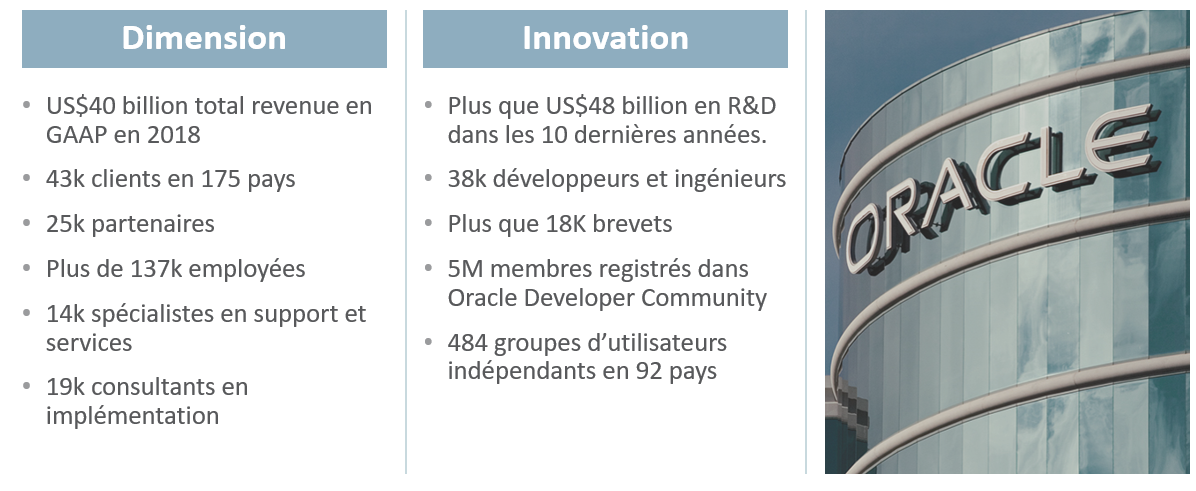
\includegraphics[width=0.8\textwidth]{chapitre1/Figures/OracleNumbers.PNG}
  \caption{Oracle, dimension et innovation}
\end{table}

\subsection{Leadership d'Oracle}
Oracle est considéré leader mondiale dans ces domaines :
\begin{table}[h!]  
  \centering
    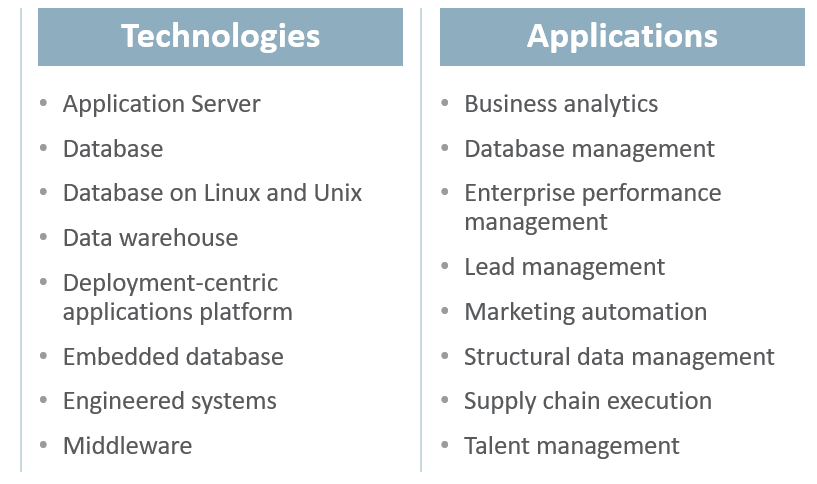
\includegraphics[width=0.8\textwidth]{chapitre1/Figures/OrcaleTechnos.PNG}
  \caption{Oracle, leader en plusieurs technologies et services}
\end{table}

\subsection{Clients Oracle}
La majorité des entreprises leader dans leur domaine, utilise des produits ou services d’Oracle.
\begin{figure}[h!]  
  \centering
    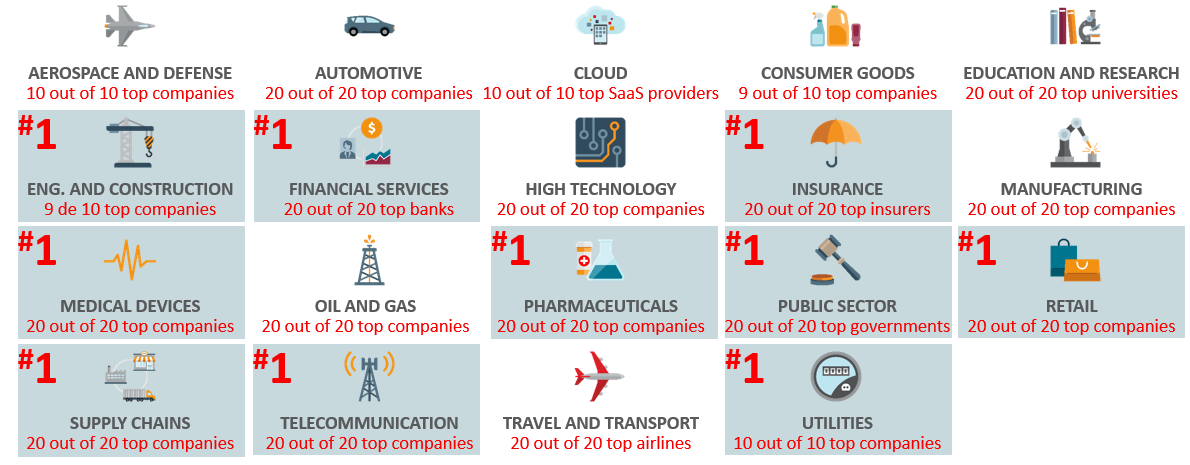
\includegraphics[width=0.8\textwidth]{chapitre1/Figures/OracleCustumers.PNG}
  \caption{Les clients d'Oracle}
\end{figure}

\subsection{Présentation de ORACLE LABS}
Oracle Labs (anciennement Sun Microsystems Laboratoires, ou Sun Labs) est une branche de recherche et développement d'Oracle Corporation. Oracle Labs a été créés lorsque Oracle a acquis Sun Microsystems [b.6].\\
\begin{figure}[H]  
  \centering
    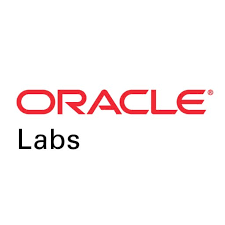
\includegraphics[width=0.5\textwidth]{chapitre1/Figures/OracleLabs.png}
\end{figure}
Oracle Labs et la source de plusieurs projets qui ont impacté la technologie d’aujourd’hui comme Java, Oracle Labs travaille aussi sur d’autres projets qui ont un grand potentiel de devenir l'état de l'art en quelques années, le plus connus est GraalVM [b.7].\\

GraalVM explore des nouvelles architectures pour les machines virtuelles (VM). La vision de GraalVM est de créer une seule VM qui offre des performances élevées pour tous les langages de programmation, facilitant ainsi la communication entre les programmes. Cette architecture supporte un outil unifié d'analyse des langages pour une meilleure maintenabilité et son intégration rendrait la VM omniprésente dans la pile de développement.\\

Cette nouvelle architecture des machines virtuelles est déjà utilisée par des grand sociétés tel que AliBaba vu son potentiel.\\

\begin{figure}[H]  
  \centering
    
\includegraphics[width=0.5\textwidth]{chapitre1/Figures/GraalVM.png}
  \caption{Logo GraalVM}
\end{figure}

Le second plus important projet sur lequel Oracle Labs travaille et PGX le projet dont j’étais membre dans mon stage PFE. PGX est une boîte à outils pour l'analyse des graphes qui permet à la fois d'exécuter des algorithmes tels que le PageRank sur les graphes, et d'effectuer des requêtes semblables à SQL mais sur les graphes, on détaillera dans la suite de ce rapport l’Outil PGX.